\documentclass{article}

\usepackage[T1]{fontenc}
\usepackage[polish]{babel}
\usepackage[utf8]{inputenc}
\usepackage{graphicx}
\usepackage{subcaption} 
\usepackage[margin=2cm]{geometry}
\usepackage{listings}
\usepackage{color}
\usepackage{amsmath}
\usepackage{tcolorbox}
\usepackage{systeme}

\definecolor{red}{RGB}{245, 63, 60}
\definecolor{blue}{RGB}{59, 69, 245}
\definecolor{green}{RGB}{59, 245, 117}
\definecolor{yellow}{RGB}{245, 207, 59}

\title{Raport Zadanie NUM4}
\date{25.11.2023}
\author{Tomasz Dziób}

\begin{document}
  \maketitle
  \newpage
  \section{Wstęp techniczny}
  Poniższy raport dotyczy zadania numerycznego NUM4 z listy 3. Załączony program o nazwie \textit{num4.cpp} został napisany w języku \textit{C++}, do sprawdzenia obliczeń został użyty plik \textit{check.cpp} również napisany w języku \textit{C++} z wykorzystaniem bibioteki \textit{GSL}. Aby uzyskać wykres prezentujący zależność wielkości danych wejściowych od czasu dla algorytmu z zadania \textit{num4.cpp} służy plik \textit{plot.cpp} napisany języku \textit{C++} korzystający z bibioteki \textit{GNU Plot}. Przed skompilowaniem programu należy zainstalować powyższe biblioteki.

    \subsection{Jak uruchomić program?}
    Razem z załączonymi plikami znajdziemy \textit{Makefile} który służy do
    uruchomienia programu \textit{num4.cpp} oraz \textit{check.cpp} komendą: \textit{make run}\\
    Aby uruchomić program \textit{plot.cpp} korzystamy z komendy: \textit{make runplot} \\

  \section{Nakreślenie problemu}
  Podczas rozwiązywania równań typu \textbf{Ay = b} dla niewiadomej \textit{b} napotykamy problem w postaci potrzeby odnalezienia wartości \textit{$A^{-1}$} której obliczenie jest skomplikowane obliczeniowo jak i pamięciowo. Najlepiej wykorzystać jest to co się posiada a mianowicie macierz \textit{A}.
  
  \section{Użyta metoda}
  Spoglądając na macierz \textit{A} jesteśmy wstanie odrazu w zauważyć jej chrakterytyczną budową, na diagonali 12, wstęga nad diagonalą same 7, reszta jedynki. Pozwala to nam na użycie wzoru Shermana-Morrisona:
  \begin{center}
    {\large$A^{-1}b= B^{-1} - \frac{ B^{-1}uv^TB^{-1} }{ 1 + v^TB^{-1}u }$}, \qquad gdzie $A = uv^T + B$
  \end{center}
  Z pomocą tego wzoru jesteśmy wstanie rozwiązać cały problem w czasie złożoności \textit{O(N)}. Najpierw \textbf{macierz A} rozpisujemy na wartości \textbf{u}, \textbf{$\mathbf{v^T}$} oraz \textbf{macierz B}.
  \begin{center}
    $\begin{bmatrix}
      12 & 8 & 1 & 1 & 1 \\
      1 & 12 & 8 & 1 & 1 \\
      1 & 1 & \ddots & \ddots & 1 \\
      1 & 1 & 1 & 12 & 8 \\
      1 & 1 & 1 & 1 & 12 \\
    \end{bmatrix}$
    $=$ 
    $\begin{bmatrix}
      1 \\
      1 \\
      \vdots \\
      1 \\
      1 \\
    \end{bmatrix}$
    \raisebox{0.9cm}{
    $\begin{bmatrix}
      1 & 1 & \cdots & 1 & 1 \\
    \end{bmatrix}$}
    $+$
    $\begin{bmatrix}
      11 & 7 & 0 & 0 & 0 \\
      0 & 11 & 7 & 0 & 0 \\
      0 & 0 & \ddots & \ddots & 0 \\
      0 & 0 & 0 & 11 & 7 \\
      0 & 0 & 0 & 0 & 11 \\
    \end{bmatrix}$
  \end{center}
  Następnie możemy zastosować podstawienie we wzorze aby uzyskać dwa równania.
  \begin{center}
    {\large$A^{-1}b= B^{-1} - \frac{ B^{-1}uv^TB^{-1} }{ 1 + v^TB^{-1}u }$} \qquad $\slash \cdot b$   \\
    \raisebox{-0.5cm}{{\large$A^{-1}b= B^{-1}b - \frac{ B^{-1}uv^TB^{-1}b }{ 1 + v^TB^{-1}u }$}} \\
    \raisebox{-0.75cm}{{\large$A^{-1}b= \textcolor{blue}{B^{-1}b} - \frac{ \textcolor{red}{B^{-1}u}v^T\textcolor{blue}{B^{-1}b} }{ 1 + v^T\textcolor{red}{B^{-1}u} }$}} \\
    \raisebox{-0.75cm}{{\Large$A^{-1}b= \textcolor{blue}{z} - \frac{ \textcolor{red}{q}v^T\textcolor{blue}{z} }{ 1 + v^T\textcolor{red}{q}}$}} \\

  \[
  \begin{aligned}
      \begin{cases}
        \textcolor{blue}{z} = B^{-1}b \\
        \textcolor{red}{q} = B^{-1}u
      \end{cases}
  \end{aligned}
  \]
\end{center}
  Pozostaje nam rozwiaząć dwa równania umieszczone poniżej używając rozkładu \textit{LU} macierzy wstęgowej poprzez \textit{forward substitution} oraz \textit{back substitution}, da się to osiągnąć w czasie \textit{O(N)}. Pozostałe operacje to oblicznie iloczynu skalarnego, mnożenie wektorów przez skalar czy odejmowanie wektorów. Wszystkie do obliczania w tej samej złożoności czasowej. 
  \begin{center}
  \[
  \begin{aligned}
      \begin{cases}
          Bz = b \\
          Bq = u
      \end{cases}
  \end{aligned}
  \]

  \end{center}



  \section{Uzyskany wynik}
  Obliczenia wykonane z użyciem algorytmu \textit{Shermana-Morrisona} pokrywa się z wynikiem uzyskanym z pojedynczego wywołania komendy \textit{solve} w bibiotece \textit{GSL}.
    \begin{flushleft}
      $\bullet$ Wynik obliczony przez program \textit{num4.cpp}
    \end{flushleft}

    \begin{center}
      \begin{tcolorbox}
        Wektor y:\\
        0.0508187 0.0508187 0.0508187 0.0508187 0.0508187 0.0508187 0.0508187 0.0508187 0.0508187 0.0508187 0.0508187 0.0508187 0.0508187 0.0508187 0.0508187 0.0508187 0.0508187 0.0508187 0.0508187 0.0508187 0.0508187 0.0508187 0.0508187 0.0508187 0.0508187 0.0508187 0.0508187 0.0508187 0.0508187 0.0508187 0.0508187 0.0508187 0.0508187 0.0508187 0.0508187 0.0508187 0.0508187 0.0508187 0.0508187 0.0508187 0.0508187 0.0508187 0.0508187 0.0508187 0.0508187 0.0508188 0.0508187 0.0508188 0.0508187 0.0508188 0.0508187 0.0508188 0.0508186 0.050819 0.0508183 0.0508194 0.0508178 0.0508203 0.0508163 0.0508226 0.0508127 0.0508282 0.0508039 0.0508421 0.050782 0.0508765 0.050728 0.0509614 0.0505946 0.0511709 0.0502653 0.0516885 0.0494521 0.0529664 0.0474439 0.0561221 0.0424849 0.0639148 0.0302393 0.0831579
      \end{tcolorbox}

      \begin{flushleft}
        $\bullet$ Wynik obliczony przez program \textit{check.cpp}
      \end{flushleft}

      \begin{tcolorbox}
        Wektor y:\\
        0.0508187 0.0508187 0.0508187 0.0508187 0.0508187 0.0508187 0.0508187 0.0508187 0.0508187 0.0508187 0.0508187 0.0508187 0.0508187 0.0508187 0.0508187 0.0508187 0.0508187 0.0508187 0.0508187 0.0508187 0.0508187 0.0508187 0.0508187 0.0508187 0.0508187 0.0508187 0.0508187 0.0508187 0.0508187 0.0508187 0.0508187 0.0508187 0.0508187 0.0508187 0.0508187 0.0508187 0.0508187 0.0508187 0.0508187 0.0508187 0.0508187 0.0508187 0.0508187 0.0508187 0.0508187 0.0508188 0.0508187 0.0508188 0.0508187 0.0508188 0.0508187 0.0508188 0.0508186 0.050819 0.0508183 0.0508194 0.0508178 0.0508203 0.0508163 0.0508226 0.0508127 0.0508282 0.0508039 0.0508421 0.050782 0.0508765 0.050728 0.0509614 0.0505946 0.0511709 0.0502653 0.0516885 0.0494521 0.0529664 0.0474439 0.0561221 0.0424849 0.0639148 0.0302393 0.0831579
      \end{tcolorbox}
    \end{center}
    Patrząc na wykres uzyskany z pliku \textit{plot.cpp} widzimy zachowanie wyników dla algorytmu \textit{Shermana-Morrisona}. Każda operacja została wykonana \textit{20000 razy} aby uśrednić wynik i zmniejszyć wpływ czynników zewnętrznych takich jak inne procesy działające w tle. Wzraz ze wzrostem danych czas wykonania omawianego algorytmu obeswujemy liniową złożoność czasową. Jesteśmy wstanie zaobserowować, mimo dużego uśrednienia, wciąż pojawiający się szum wzrastający równo z ilością danych wejściowych.
    \begin{figure}[!ht]
      \centering
      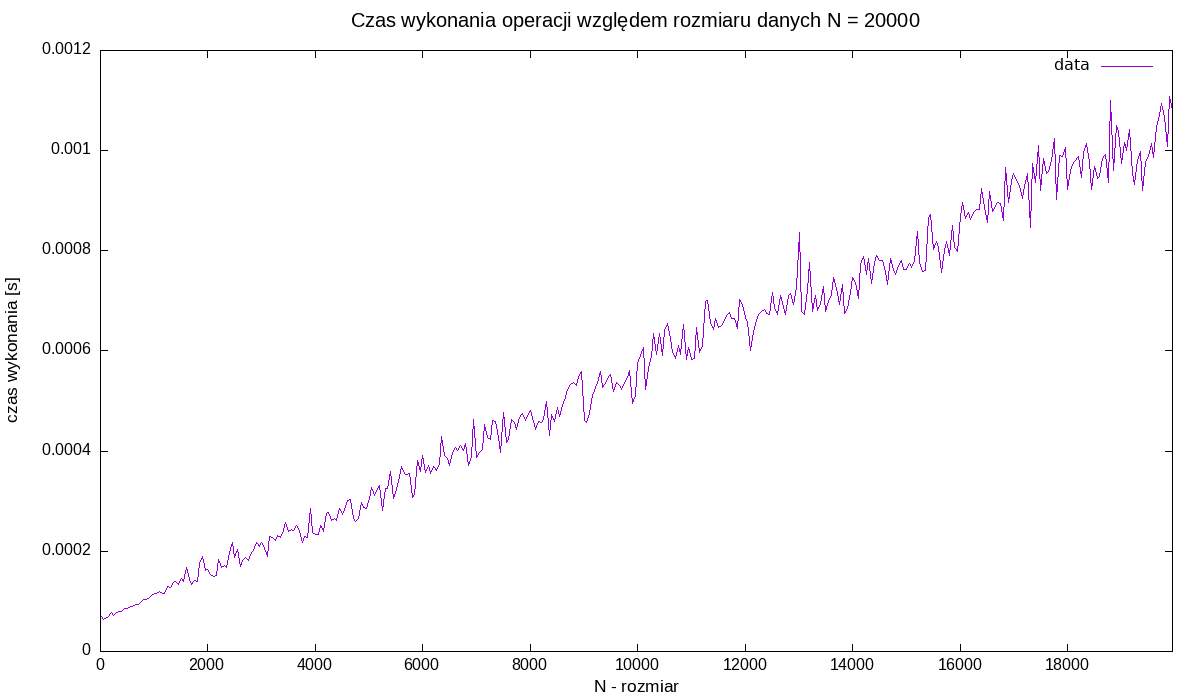
\includegraphics[width=0.66\linewidth]{wyniki.eps}
      \caption{Wynik uzyskany po uruchomienu programu \textit{plot.cpp}}
    \end{figure}
    \newpage
  \section{Podsumowanie}
  Wzór Shermana-Morrisona sprawuje się idealne w przypadku potrzeby obliczenia odwrotności macierzy jeśli jesteśmy tylko wstanie wyrazić ją jako wynik $uv^T + B$. Jest to operacja o wiele prostsza od znajdywania odwrotności macierzy. Wykonanie jej wiąże się również z polepszoną złożonością czasową. 
\end{document}